\documentclass[12pt]{article}
\input{/Users/circle/Documents/博一下/homework/setting.tex}
\setcounter{secnumdepth}{2}
\usepackage{autobreak}
\usepackage{amsmath}
\setlength{\parindent}{2em}
\graphicspath{{../}}
\ziju{0.1pt}

%pdf文件设置
\hypersetup{
	pdfauthor={袁磊祺},
	pdftitle={高等实验流体力学大作业}
}

\title{
		\vspace{-1in} 	
		\usefont{OT1}{bch}{b}{n}
		\normalfont \normalsize \textsc{\LARGE Peking University}\\[0.2cm] % Name of your university/college \\ [25pt]
		\horrule{0.5pt} \\[0.2cm]
		\huge \bfseries{高等实验流体力学大作业} \\[-0.2cm]
		\horrule{2pt} \\[0.2cm]
}
\author{
		\normalfont 								\normalsize
		College of Engineering \quad 2001111690  \quad 袁磊祺\\	\normalsize
        \today
}
\date{}

\begin{document}

\input{/Users/circle/Documents/博一下/homework/setc.tex}

\maketitle

代码和文档可以在 \href{https://github.com/circlelq/Advanced-Experiment-Fluid-Mechanics}{https://github.com/circlelq/Advanced-Experiment-Fluid-Mechanics} 查看。

\section{PIV课程设计}

\subsection{课程设计目标}

完成一个二维PIV技术的基本系统设计,对图像处理、基本算法有初步、较为清晰的理解。

\subsection{课程设计内容}

设计内容主要涉及以下内容:PIV原始图像的获取、PIV图像的计算框架、PIV图像相关算法、二维PIV数据可视化



\subsection{课程设计中的若干问题说明}


\begin{enumerate}
	\item 原始图像的获取: 推荐三种建立原始图像的路径:
	      \begin{enumerate}
		      \item 图像仿真方法:随机建立粒子像的中心坐标,形成高斯光斑,确定光斑光强,按照3*3像素或5*5离散,确认 粒子数密度(建议达到$0.1 \sim 0.2$PPP(Particle Per Pixel),按照某种流动规律,生成第二幅曝光粒子图像。可以考 虑加入随机噪声。
		      \item 简易PIV系统:利用手机摄像机,对一个慢速运动成像,如:水盆中漂浮的缓慢运动的泡沫颗粒.
		      \item 实验室装置:可以自行设计一个简易模型,利用实验室PIV设备进行测试,获取图像。
	      \end{enumerate}
	\item PIV图像处理和计算: 了解图像格式、图像前置处理、相关算法、相关峰值的亚像素拟合计算、偶然误差处理。
	\item 二维PIV数据可视化:利用TECPLOT形成速度矢量场、梯度场等。
\end{enumerate}


\section{数据获取}

我和王博源同学一起去圆明园校区进行了实验(之后的报告和数据处理是独立完成的),实验装置是一个水槽,水槽内的水均匀流动。水槽下方有一束激光向上照射,打在水中的示踪粒子上形成点状图像,并用相机从水平方向上进行拍摄,如\cref{fig:1} 所示,为拍摄样片,可以发现白色的粒子点非常清晰,背景没有杂色,所以这里省去了图片预处理。

\begin{figure}[htp]
	\centering
	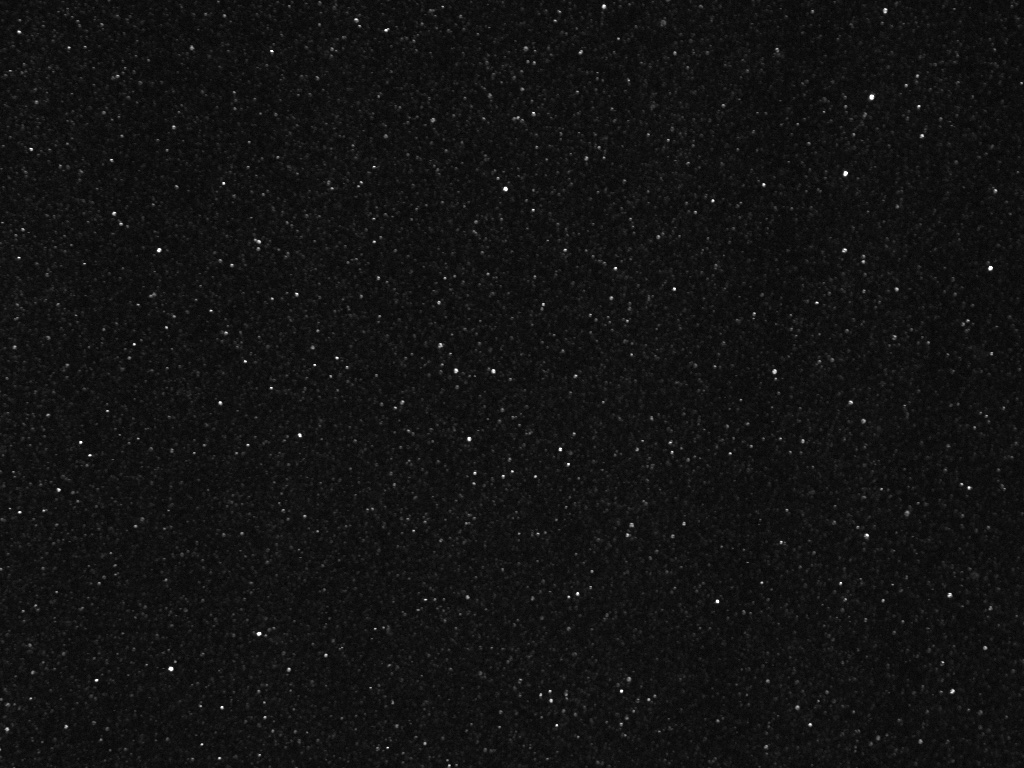
\includegraphics[width=10cm]{001}
	\caption{拍摄样片。}
	\label{fig:1}
\end{figure}

采样频率为2000Hz。通过尺子进行标定可得$(219,28),\ (201,633)$两个像素点间的距离是20mm。所以,两个相邻像素点的距离是
\begin{equation}
	h = \frac{20 \mathrm{mm}}{\sqrt{\left(219-201\right)^2+\left(28-633\right)^2}} = 0.0330 \mathrm{mm}.
\end{equation}



\section{数据处理}

\cref{fig:1} 的格式是\texttt{.tif},标签图像文件格式(Tagged Image File Format,简写为TIFF)是一种灵活的位图格式,主要用来存储包括照片和艺术图在内的图像。通过Matlab的\texttt{imread()}读取图片。

将interrogation areas的宽度设为20,在上下左右10个像素点的距离计算相邻两帧图片的二维相关函数
\begin{equation}
	r=\frac{\sum_{m} \sum_{n}\left(A_{m n}-\bar{A}\right)\left(B_{m n}-\bar{B}\right)}{\sqrt{\left(\sum_{m} \sum_{n}\left(A_{m n}-\bar{A}\right)^{2}\right)\left(\sum_{m} \sum_{n}\left(B_{m n}-\bar{B}\right)^{2}\right)}},
\end{equation}
画图可得\cref{fig:2}.可以发现相关性较大的点非常明显,所以之间将相关系数最大的点作为粒子团新的坐标点,并计算移动的位置,记录在\texttt{vec}数组里。

\begin{figure}[htp]
	\centering
	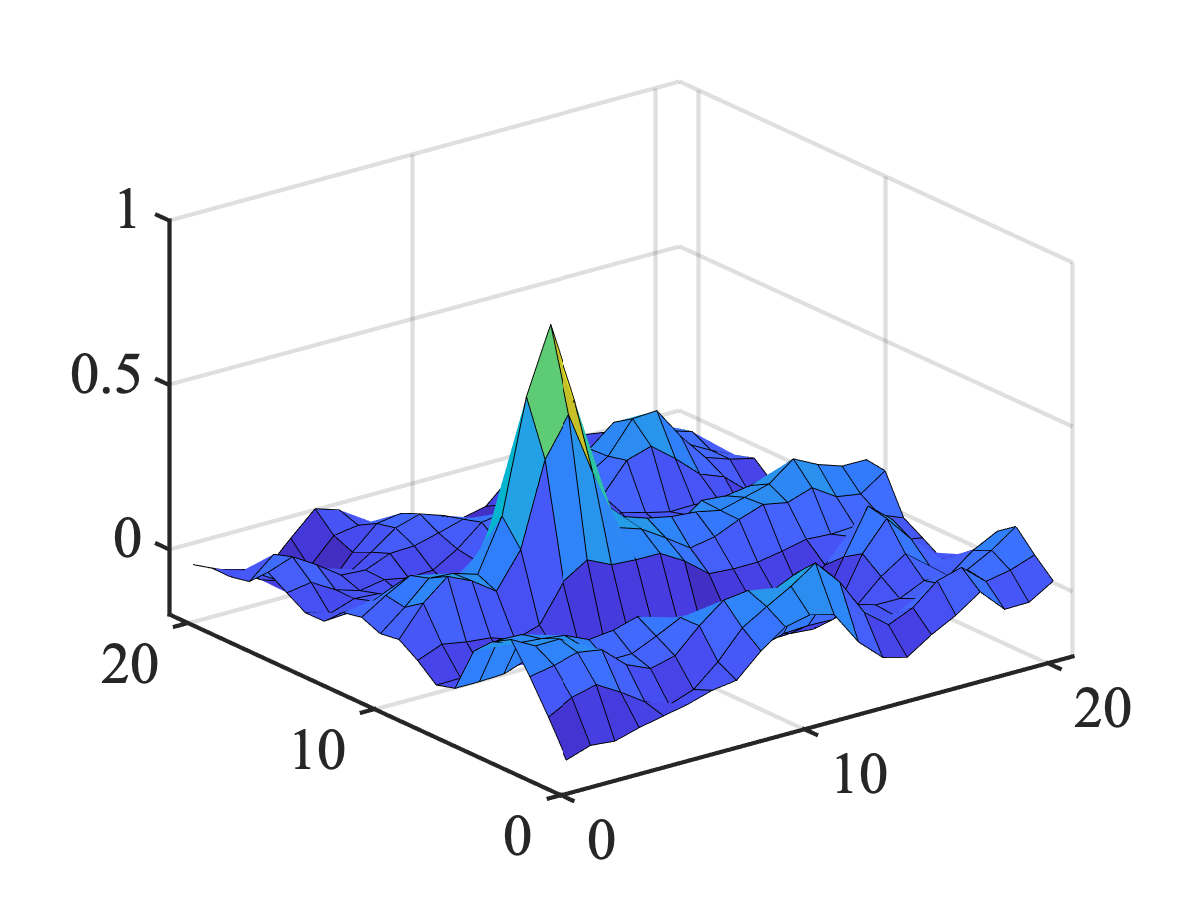
\includegraphics[width=10cm]{corr}
	\caption{附近点的相关函数。}
	\label{fig:2}
\end{figure}

如\cref{fig:3} 所示,流场为均匀场,经过一个时间点后移动的位置为三个像素点。流速为
\begin{equation}
	u = \frac{3h}{\tau} = \frac{3\times 0.0330 \mathrm{mm}}{1/2000 \mathrm{s}} = 20 \mathrm{cm/s}.
\end{equation}

\begin{figure}[htp]

	\centering
	\begin{subfigure}[b]{0.49\textwidth}
		\centering
		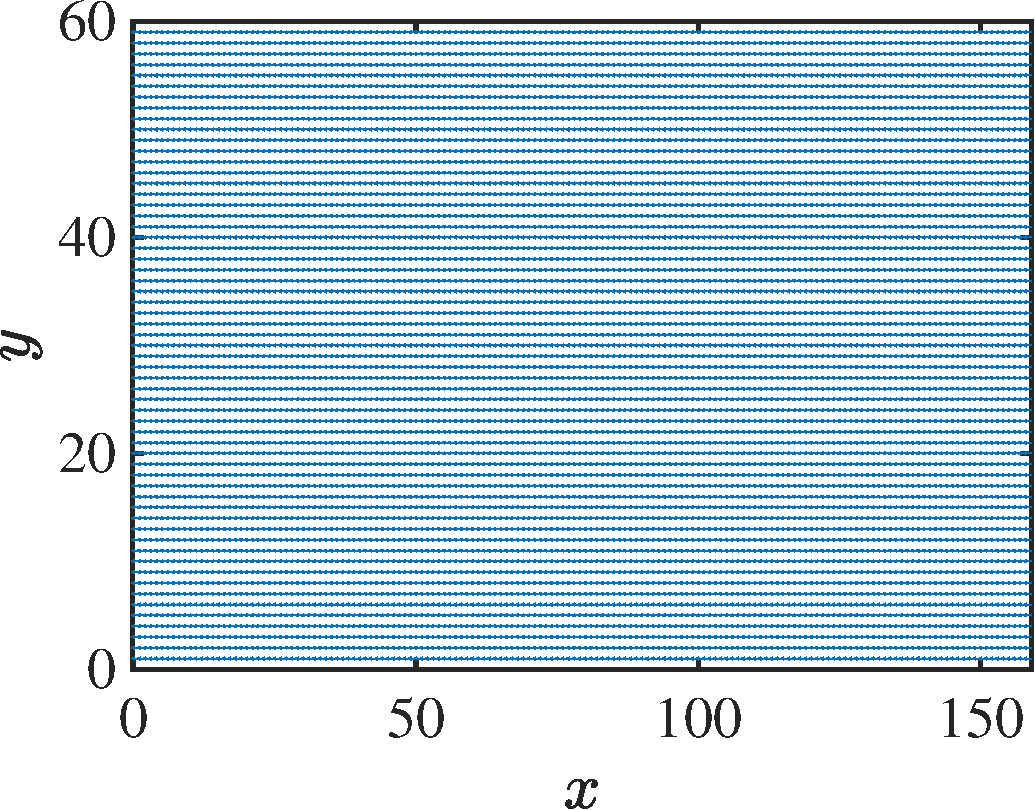
\includegraphics[width=7cm]{Velocity.pdf}
		\vspace{0.35cm}
		\caption{流场向量场。}
	\end{subfigure}
	\hfill
	\begin{subfigure}[b]{0.49\textwidth}
		\centering
		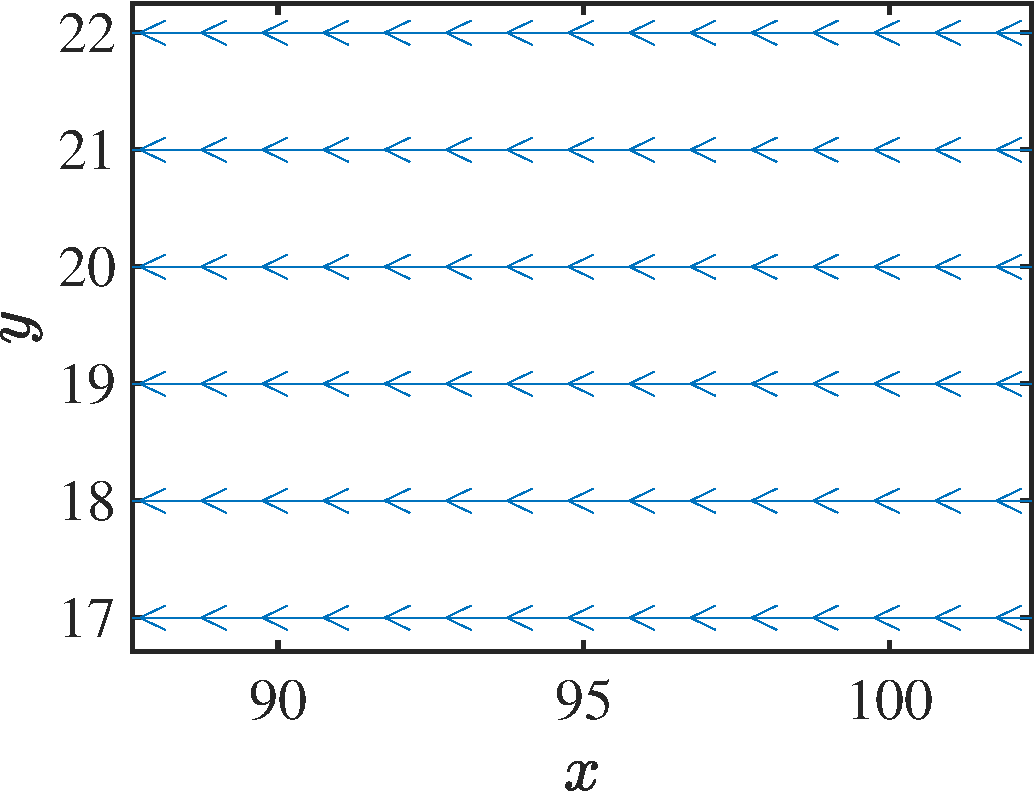
\includegraphics[width=7cm]{VelocityMag.pdf}
		\vspace{0.35cm}
		\caption{流场向量场放大。}
	\end{subfigure}
	\caption{流场向量场。}
	\label{fig:3}
\end{figure}

\section{代码}

\begin{lstlisting}[language=Matlab]
I1 = imread('001.tif');
I2 = imread('002.tif');

I1 = I1(1:100, 1:200);
I2 = I2(1:100, 1:200);

width = 20; % the width of interrogation areas
d = ceil(width/2);
l = 10; % search interrogation areas no longer than l

[m, n] = size(I1);

vec = zeros(m-2*l-2*d-2, n--2*l-2*d-2, 2);
corre = zeros(2*l+1, 2*l+1);

for i = l+d+1:m-d-l-1
	for j = l+d+1:n-d-l-1
		for p = -l:l
			for q = -l:l
				% calculate correlation
				corre(p+l+1, q+l+1) = corr2(I1(i-d:i+d, j-d:j+d), I2(i+p-d:i+p+d, j+q-d:j+q+d));
			end
		end
		% surf(corre)
		[M, index] = max(corre);
		[M1, index_j] = max(M);
		index_i = index(index_j);
		vec(i-l-d, j-l-d, 2) = index_i-l-1;
		vec(i-l-d, j-l-d, 1) = index_j-l-1;
	end
end
\end{lstlisting}


% \nocite{*}

% \bibliographystyle{plain}

\phantomsection

\addcontentsline{toc}{section}{参考文献} %向目录中添加条目,以章的名义
\bibliography{homework}

\end{document}

